\section{Semantic web}

\subsection{Implicit vs.\ explicit knowledge}
Information retrieval data mining aim at extracting knowledge that is
implicitly represented in documents. But knowledge can also be
explicitly represented.

\subsection{Semi-structured data}
\subsubsection{Database schema}
\textbf{Schemas} define data structures for databases
\begin{itemize}
\item Relational schemas, XML schemas
\end{itemize}
Agreement on data structures
\begin{itemize}
\item Well understood interpretation of data values
\item Data consistency
\end{itemize}
Optimizing query evaluation and data storage
\begin{itemize}
\item Schema fragmentation for distributed databases
\end{itemize}

\subsection{Data on the web}
Typical approach is to use HTML to structure data. In this way a
context is provided, that allows to correctly interpret data
values. Problem is HTML has never been conceived to \textbf{specify
  semantics of data}.

\subsection{Application-specific markup}
Limitations of HTML:
\begin{itemize}
\item Structure of data expressed as layout: <tr><td>leech</td></tr>
\item Semantics of data hard to analyse and difficult to share
\item No schemas, no constraints
\end{itemize}

Making the meaning of data explicit
\begin{itemize}
\item SwissProt: <Species> leech </Species>
\item EMBLChange: <Organism> leeach </Organism>
\end{itemize}

Embedding of schema information into the data

\subsection{Semi-structured data}
Data that contains tag, markup or similar to specify the semantics of
data values and to relate different data values. No predefined
structure, no schema required!

Examples:
\begin{itemize}
\item EMail
\item Microformats (e.g.\ hCard)
\item JSON
\item XML (document and data model)
\end{itemize}

A serialized document is a medium of exchange of information

\subsection{Schema-less data}
\textbf{Benefits}
\begin{itemize}
\item Increased flexibility (dynamically adding or dropping attributes
  or structure)
\item Self-contained data: context directly encoded into data (markup)
\end{itemize}
\textbf{Drawbacks}
\begin{itemize}
\item Loss of consistency
\item Certain optimizations not feasible
\end{itemize}

\subsection{The semantic web}
User-defined markup (schemas): provides possibility to share
interpretation of data accross various applications.

Different databases - Different schemas
\begin{itemize}
\item Swissprot
\item EMBLChange (see above)
\end{itemize}

Problem: Semantic heterogeneity $ \rightarrow $ semantic web. \\
XML can be interpreted by applications but to properly do it semantic
heterogeneity needs to be overcome as well. The same concepts can (and
will be) represented in different application context differently (by
using different names). This is a major obstacle to enable
interoperability on the Web.

\subsubsection{The vision of W3C}
To address this problem, the W3C launched the semantic web
initiative. It is a framework that builds on web technology, including
XML, and extends it with technologies that facilitate semantic
interop.

\subsubsection{Three ways to overcome semantic hetero}
\begin{itemize}
\item Standardisation: agree on common markup
  \begin{itemize}
  \item Great if no pre-existing applications
  \item Great if power player enforces it
  \end{itemize}
\item Translation: create mapping among different schemas and
  databases
  \begin{itemize}
  \item requires human interpretation and reasoning
  \item mappings can be difficult, expensive to establish
  \end{itemize}
\item Annotation: create relationships to agree upon conceptualization
  \begin{itemize}
  \item requires human interpretation and reasoning
  \item annotations can be difficult, expensive to establish
  \item reasoning over the conceptualization can provide added value
  \end{itemize}
\end{itemize}

\subsection{Annotation}
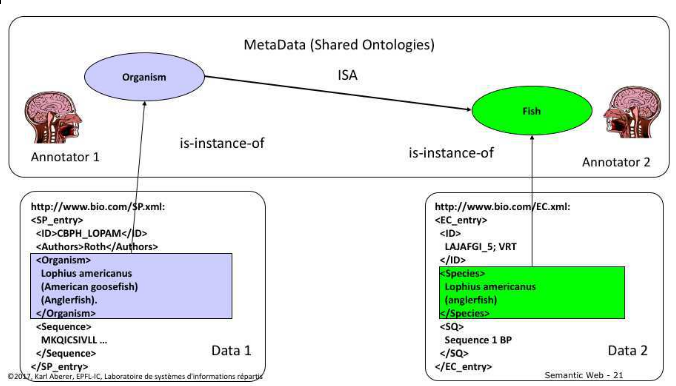
\includegraphics[width=200px, height=100px]{annot}

\subsection{Ontologies}
Explication specification of a conceptualization of the real world \\
Ideally
\begin{itemize}
\item different information systems agree on the same ontology
\item relate their model/schema/data elements to the ontology
\item mapping can be constructed via the ontology
\end{itemize}

Requires agreement on the ontology! Ontologies provide ``proxy
representation'' for the real world.

\subsubsection{Creating ontologies}
Ontology engineering
\begin{itemize}
\item Manual effort
\item Tools for editing and checking consistency
\end{itemize}

Automatic induction of ontologies
\begin{itemize}
\item From large doucment collections or existing structured resources
\end{itemize}

\subsubsection{Modeling and encoding}
Issue
\begin{itemize}
\item Modeling primitives and their semantics: what does an arrow
  mean? what does ``instance-of'' mean? \ldots
\item Different encoding of the model
\end{itemize}

\subsubsection{Model requirements}
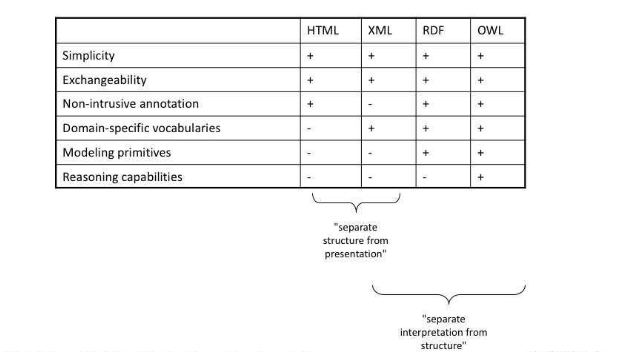
\includegraphics[height=100px, width=200px]{modelreq}

\begin{itemize}
\item Simplicity: Success of the web is based on simplicity: complex
  model will not be successful!
\item Exchangeability: the web is a communication environment, any
  data must be easily exchangeable.
\item Non-intrusive annotation: machine-processable knowledge is
  usually will be added a-posteriori. Thus any attempt to encode the
  knowledge directly into data is not practical
\item Domain-specific vocabulary: the model must provide a mechanism
  that permits to introduce terminology that is specific to a domain
\item Modeling primitives
\item Reasoning capabilities: any form of reasoning can make the
  interpretation of the data much more powerful
\end{itemize}

\subsection{RDF}
RDF (instances)
\begin{itemize}
\item Statements about Resources (addressable by URI) and literals
  (XML Data)
\item Statement are of the form: subject property object
\item Like simple natural language sentences
\item RDF statements are themselves resources (reasoning about RDF)
\item Properties define relationships to other resources or atomic
  values
\end{itemize}

RDF-schema
\begin{itemize}
\item Data model to specify schemas for RDF instances
\item Which properties are application for which objects with which
  subjects
\item Defines ``grammar'' and ``vocabulary'' for semantic domains
\item Similar to entity-relationship model
\end{itemize}

RDF is used to annotate XML documents.

\subsubsection{RDF statements}
Basic constituents of RDF\. Can be seen as
\begin{itemize}
\item natural language sentences where subject is an URI and the
  object is either a URI or a String
\item directed graph where the subject and object are nodes and the
  predicate is a directed link
\item XML documents where statement is encoded in XML format
\end{itemize}

The graph representation is well-suited for reasoning and
visualization and XML format used for exchange and storage

\subsubsection{RDF syntax}
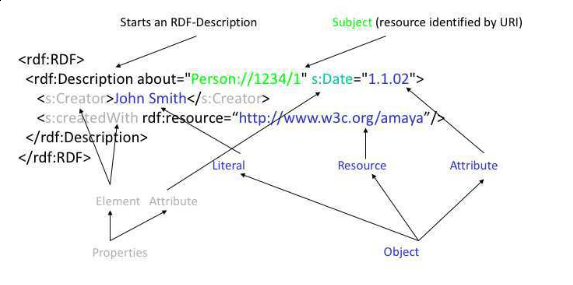
\includegraphics[width=200px, height=150px]{rdfsynt}

Resource can be typed by using \textbf{rdf:type}

\subsubsection{RDF complex values}

Associating a subject with a property whose value is a simple object
is the simplest form of statement. In order to represent complex
object a new intermediate resouce is created to which different
properties are associated. Not that this is diffirent of directly
associating these properties with the subject of the overall
statement.\\
In XML encoding such a complex value can be represented by directly
inlining the complex object into the statement.

\subsubsection{RDF containers}
Containers
\begin{itemize}
\item Bag (unordered)
\item Seq (ordered)
\item Alt (alternatives)
\end{itemize}

Quantifiers
\begin{itemize}
\item about: John is author of the talk (containing many slides)
\item aboutEach: John is author of each of the slide of the talk
\end{itemize}

Containers are special resources. A container is associated with a set
of other resources (the content of the container). By creating a
statement using the container as object, one can express
statements made about the set of objects. One can specify whether the
statement is about the set of object as a whole, or about each element
of the set individually (consequences of distinction: \textbf{not
  specified}!). The set order can be imposed by using labels \_1, \_2,
\ldots. If order is irrelevant use label rdf:li instead.


\subsubsection{Creating new resources}
\begin{itemize}
\item Created using \textbf{rdf:ID} property
\item A new resources can be defined by having rdf:ID replace the
  rdf:about property. \textbf{rdf:about} references another object and
  \textbf{rdf:ID} signifies resource creation and definition
\end{itemize}

\subsubsection{RDF reification}
\begin{itemize}
\item Statements on RDF statements (commenting, disputing, \ldots)
\item In RDF everything is a resource so should be able to make
  statements about everything
\item Not clear when using graph representation
\end{itemize}

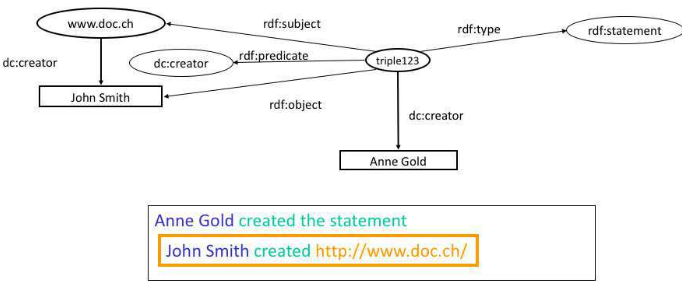
\includegraphics[width=220px, height=100px]{reification}

\subsubsection{RDF reification syntax}
The statement has an anonymous resource as subject, namely the reified
statement which is fully defined by its properties.

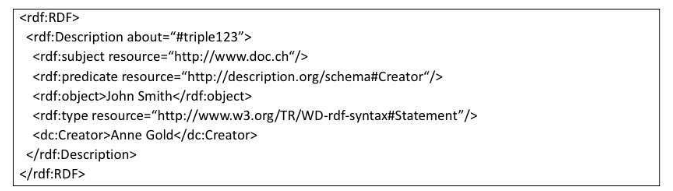
\includegraphics[width=220px, height=80px]{reificationsynt}

\subsubsection{RDF schema classification}

RDF resources
\begin{itemize}
\item anything that can be described
\end{itemize}
RDF classes
\begin{itemize}
\item Categories for subjects and objects
\item Classes allow to associate a type with and RDF instance
\item Different classes can be in a subClass relationship
\item Classes are RDF instances
\end{itemize}
RDF schema mechanisms
\begin{itemize}
\item Categorizations of RDF resources
\item Constraints on the use of properties, sort of a type system!
\item Classses are resources, which are of type rdfs:Class
\end{itemize}

\subsubsection{RDF schema - properties}
RDF properties: \texttt{connect resources}
\begin{itemize}
\item The rdf instance must have the properties that are declared for
  the class
\item rdfs:domain: classes of which the instances may have a property
\item rdfs:range: classes of which the instance may be the value of a
  property
\item contstrains the use of properties that connect resources
\item they are represented as resources
\end{itemize}

Example: marital status
\begin{itemize}
\item In RDF schema it is possible to constrain the usage as follows
\item by connecting the property resource through the property
  rdfs:domain to a class resource, one specifies that the subject when
  using this property must originate from that class
\item Similarly for the object, the range can be constrained using
  rdfs:range
\end{itemize}

XML serialization
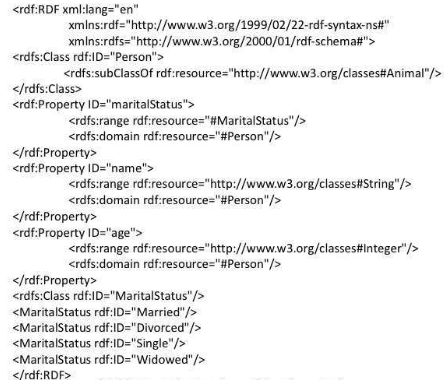
\includegraphics[width=200px, height=200px]{rdfsxml}

\subsubsection{Schema inheritance}
rdfs:subClassOf
\begin{itemize}
\item A subClassOf B: every instance of A is also an instance of B
\item transitive, not-reflexive, anti-symmetric
\item M:N: a class can have arbitrarily many subclasses and
  superclasses
\item Subclass has all properties of the superclass
\end{itemize}

rdfs:subPropertyOf
\begin{itemize}
\item P1 subPropertyOf P: if A has Property P1 with B then it also has
  value B with Property P2
\item Example: Anne has property Father with value John, and Father
  subProperty AParent implies Anne has Property AParent with value John
\end{itemize}

\subsection{Semantic web resources}

\subsubsection{WordNet}
English dictionary with semantic relationships
\begin{itemize}
\item \textbf{Synonymy}: words that have similar meanings
\item \textbf{Antonymy}: opposite of synonymy
\end{itemize}
Nouns only
\begin{itemize}
\item \textbf{Hypernymy}: Hierarchical relationship between words,
  i.e.\ furniture is a hypernym of chair since a chair is a piece of
  furniture
\item \textbf{Hyponymy}: Opposite of hypernymy. Dog is a hyponym of
  canine since every dog is a canine.
\item \textbf{Meronymy}: Part-whole relationship. Paper is a meronym
  of book, since paper is part of a book
\end{itemize}

\subsubsection{Schema.org}
Collaborative community active to create, maintain, and promote
schemas for structured data on the Internet
\begin{itemize}
\item Two type hierarchicies: textual properties values, things that
  they describe
\item Core vocabulary contains 642 types, 992 properties and 219
  enumaration values
\item Used by other knowledges bases, Google knowledge, Graph API
  \ldots
\end{itemize}

\subsubsection{Encoding}
Different encodings can be used, JSON, RDFa, Microdata. \\
RDFa: microformat for embedding RDF into HTML.
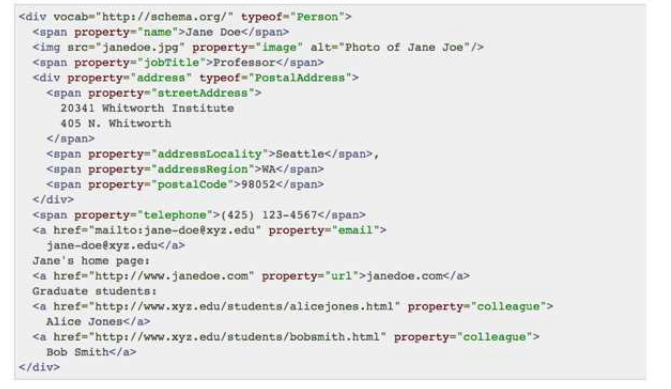
\includegraphics[width=200px, height=170px]{rdfa}

\subsubsection{WikiData}
Community project to create open database of structured data
\begin{itemize}
\item Data curation like wikipedia
\item Intented to support wikipedia
\item 16.5+ million statements
\item Multi-lingual
\item Both API access and full databases dumps
\end{itemize}

\subsubsection{Google Knowledge Graph}
Google's internal knowledge base to support search engine
\begin{itemize}
\item Populated from FreeBase and internal data
\item Enriched with the support of schema.org
\item Accessible through API
\end{itemize}

\subsection{Ontology languages}
Limitations of RDF schema
\begin{itemize}
\item Limited expressive power (subclass, property, subproperty)
\item Unclear semantics (subproperty never precisely defined)
\item No reasoning support
\end{itemize}

Requirements of ontology languages
\begin{itemize}
\item Well \textbf{designed}
  \begin{itemize}
  \item Intuitive to human users
  \item Adequate expressive power
  \end{itemize}
\item Well \textbf{defined}
  \begin{itemize}
  \item Clearly specified syntax
  \item Formal \textbf{semantics}
  \item Adequate expressive power
  \end{itemize}
\item Compatbile with existing web standards
  \begin{itemize}
  \item in particular RDF
  \end{itemize}
\end{itemize}

\subsection{OWL (Web ontology language)}
Developed to match these criteria. Unifies ideas from earlier
developments and fields.
\begin{itemize}
\item \textbf{Description logics} describes knowledge in terms of
  concepts and role restrictions that are used to derive
  classification taxonomy. OWL inherits from DL its formal semantics
  and the efficient reasoning support
\item \textbf{Frame-based systems} provide as central modeling
  primitives classes with attributes. These attributes do not have a
  global scope but are only applicable to the classes they are defined
  for. A frame provides a certain context for modeling one aspect of a
  domain. OWL incorporates the essential modeling primitives of those
  systems.
\item \textbf{Web standards: XML and RDF}: provide web standards for
  representation and exchange. OWL uses these as follows:
  \begin{itemize}
  \item OWL has a well-defined syntax in XML based on a document type
    definiton
  \item OWL is an extension of RDF and RDFS
  \end{itemize}
\end{itemize}

\subsubsection{OWL as RDF extension}
The languague to specifiy OWL models is given as an RDF schema
\begin{itemize}
\item like the RDF schema language is expressed within an RDF schema
\item there OWL models can be expressed in RDF
\item some of the OWL modeling primitives and RDF modeling primitives
  overlap and are re-used in IWL
\end{itemize}
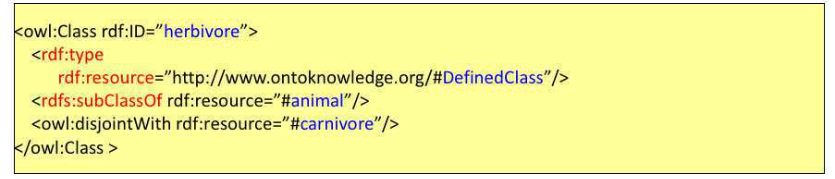
\includegraphics[width=200px, height=40px]{owl}

\subsubsection{OWL semantics}
The semantics of OWL is given in Description Logics (DL)
\begin{itemize}
\item Description logics is a fragment of first order predicate logic
\item reasoning can be done more efficiently  than in first order
  predicate logic
\end{itemize}

\subsubsection{Property semantics in OWL}
Classes in OWL (RDF) are \texttt{unary} predicate \\
Slot constraints (=properties) in OWL are \texttt{binary} predicates
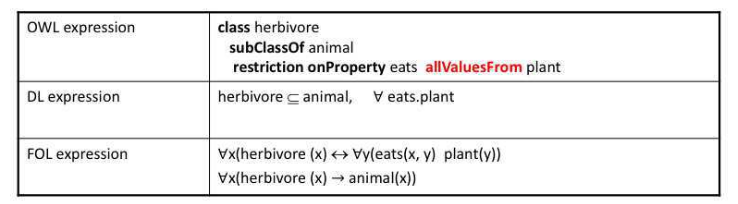
\includegraphics[width=200px, height=80px]{owlsemantics}

%%% mode: latex
%%% TeX-master: "master"
%%% End:
\item
